\documentclass[12pt, a4paper]{article} %Definerer skriftstørrelse, arktrype( eks a0paper, ..., a6paper, letterpaper....), dokumenttype(article, report, book, letter, beamer(presentasjon).   
\usepackage[font=small, labelfont=bf]{caption}
\usepackage{graphicx}
\usepackage{pdfpages}
\usepackage{amsmath, amssymb} %  matematiske funskjoner og symboler. 
\usepackage{listings}
\usepackage{url} % urls in the bibliograpy
\usepackage[utf8]{inputenc} % 
\usepackage{float}  %
\usepackage{subcaption} % NOT compatible with the subfig package
\usepackage{authblk}
\usepackage{siunitx}
\usepackage[parfill]{parskip}


\usepackage[  
left=20mm,
 right=20mm,
 top=10mm,
 bottom=20mm]{geometry} % kan endre på marger 
%%%%%%%%%%%%%%%%%%%%%%%%%%%%%%%%%%%%%%%%%%%%%%%%%%%%%%%%%%%%%%%%
% Gode infosider:
% https://no.sharelatex.com/learn/Creating_a_document_in_LaTeX 
% https://no.sharelatex.com/learn/Page_size_and_margins
 
%%%%%%%%%%%%%%%%%%%%%%%%%%%%%%%%%%%%%%%%%%%%%%%%%%%%%%%%%%%%%%%%
% Det som inkluderes i \maketitle
\title{Øving 2\\ TDT4200}
\author[1]{Anette Fossum Morken og Vanje Rebni Kjer}
\date{}
%%%%%%%%%%%%%%%%%%%%%%%%%%%%%%%%%%%%%%%%%%%%%%%%%%%%%%%%%%%%%%%
\begin{document}
\maketitle

\section*{Del 1, oppgave 1}
\subsection*{a}
\subsubsection*{i)}
Nvidia Maxwell er en arkitektur for GPU-er, der en GPU er bygd opp av $ 8$, $16 $ eller $ 24 $ streamingmultiprosessorer (SM). Hver SM har $ 128 $ homgene kjerner,der hver SM kan behandle opptil $ 2000 $ tråder.
\subsubsection*{ii)}
ARM big.LITTLE er en arkitektur med heterogene kjerner som typisk er brukt i mobiltelefoner eller andre enheter der batterilevetiden er viktig. Det ene settet med kjerner er kraftigere og dermed mer energikrevende, og det andre settet med kjerner er svakere og dermed mindre energikrevende. Et eksempel er tekstbehandling, som gjøres på de mindre energikrevende kjernene og tyngre oppgaver gjøres på de mer energikrevende kjernene. Hver kjerne jobber med en tråd om gangen.

\subsubsection*{iii)}
vilje@NTNU er en superdatamaskin som er et cluster med $1404$ noder. Hver node har to prosessorer med åtte homogene kjerner, der hver kjerne har hyperthreading-kapabilitet. Dette betyr at hver kjerne kan jobbe med to individuelle tråder samtidig. Vilje bruker en NUMA-arkitektur, der hver prosessor har 16 GB RAM hver.

\subsubsection*{iv)}
En typisk CPU i dag har to, fire eller åtte homogene kjerner med hyperthreading slik at hver kjerne kan behandle to tråder samtidig. CPU-en bruker NUMA i den forstand at hver enkeltkjerne har sin egen L1- og L2-cache. 

\subsection*{b}
SIMT (Single instruction, multiple threads) ligner på SIMD i Flynns taksonomi. Her har man èn enkelt instruksjon som utføres over flere tråder. Av alle alternativene ovenfor er det kun Nvidia sin Maxwell-arkitektur som benytter SIMT. Dette er realisert ved at grupper på $ 32 $ kjerner utfører samme instruksjonssett samtidig på forskjellige data.

\subsection*{c}
\subsubsection*{i)}
Nvidia Maxwell passer best inn under SIMD i Flynns taksonomi som forklart i b).
\subsubsection*{ii)}
ARM big.LITTLE passer inn i både MIMD og SIMD i Flynns taksonomi, fordi den har mulighet til å kjøre flere instruksjonssett samtidig, f.eks. å kjøre en oppdatering samtidig som man gjør noe annet. I midlertid har den muligheter for SIMD, f.eks ved en koding/dekoding av video. MIMD passer kanskje best til å beskrive arkitekturen, fordi man ikke er låst til å kjøre en enkelt instruksjon på alle kjernene.
\subsubsection*{iii)}
For vilje@NTNU passer beskrivelsen MIMD best, fordi ulike brukere av Vilje kan kjøre helt forskjellige program uavhengig av hverandre. 
\subsubsection*{iv)}
En vanlig CPU kan passe inn under både SIMD og MIMD. Her vil forklaringen være den samme som for ARM big.LITTLE-arkitekturen.


\section*{Del 1, oppgave 2}
\subsection*{a}
En tråd er en komponent i en prosess. I Nvidia sin Maxwell-arkitektur organiseres flere tråder inn i en blokk, der hver blokk består av et visst antall tråder som kan kommunisere med hverandre. Et grid består av flere blokker som ikke kan kommunisere med hverandre. 

\section*{b}
Setter opp ligninger for tiden GPU-en vil bruke og CPU-en vil bruke:
\begin{align}
GPU=\frac{2n}{r}+\frac{5n}{r}+5h_{GPU}n7h_{GPU}log_2(n) \nonumber \\
CPU=5h_{CPU}n7h_{CPU}log_2(n)
\label{alg}
\end{align}
der $h_{GPU}=1$, $h_{CPU}=10$, $r$ er båndbredden og $n$ er mengde data som overføres. Det lønner seg å bruke GPU-en når $GPU>CPU$ det finnes ved å regne ut $GPU$ og $CPU$ for mange forskjellige $n$ og plotte dem og se hvor de krysser hverandre slik at $GPU>CPU$.
 Med den oppgitte algoritmen vil det ta kortest til å kjøre på GPUen hvis $n \geqslant 1$, dette kan sees ved å studere plottet i figur \ref{GPU-CPU}. For de fleste andre programmer er ikke dette riktig. Vanligvis vil det være raskest å kjøre programmer der $n$ er liten på CPUen siden minneoverføringen til og fra GPUen er tidkrevende. 
\begin{figure}
\centering
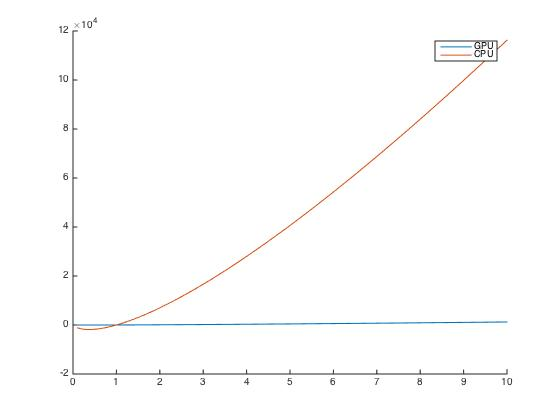
\includegraphics[width=0.5\textwidth]{GPU-CPU.jpg} 
\caption{Plottet viser kjøretiden for et program gitt med kjøretidene i \eqref{alg}}
\label{GPU-CPU}
\end{figure}

\subsection*{c}
Kernel2 vil være raskest siden her blir alle trådene satt i arbeid. I kernel1 looper man gjennom trådene og gir bare et utvalg av trådene arbeid. Hvis trådene i en warp har fått forskjellige instruksjoner vil de bli kjørt serielt og siden alle trådene ikke har samme instruksjon i kernel1 vil denne kjøres serielt. I kernel2 får alle trådene i hver blokk samme instruksjon og vil derfor kjøres parallelt.

\subsection*{d}
\subsubsection*{i)}
Warps er en samling med $ 32 $ tråder. Hvis trådene utfører samme operasjon kan de kjøres parallellt, men har de forskjellige oppgaver må de kjøres serielt. For å utnytte parallelliteten maksimalt må alle trådene i warpen ha samme instruksjon.
\subsubsection*{ii)}
Occupancy gir hvor stor prosentandel av tilgjengelige warps som er i bruk. Man kan også se på det som hvor mange av trådene som står og venter på å få arbeide. Prosentandelen bør være så høy som mulig for å få gjort mest mulig på kortest tid.
\subsubsection*{iii)}
Minnefortetting (coalescing) er å slå sammen flere minneoverføringer mellom minnet og trådene til kun èn overføring. Det gjør at et gitt antall tråder i en warp kan hente ut informasjon fra minnet på en gang, og tiden det tar for alle å hente ut informasjonen er den samme som om kun èn tråd hadde brukt om man ikke benyttet seg av coalescing. På denne måten kan man redusere kjøretiden til programmet.
\subsubsection*{iv)}
Lokalt minne er minne som en tråd kun har tilgang til. Skal en tråd ha informasjon fra en annen, må dette deles gjennom message passing.
\subsubsection*{v)}
Delt minne er at alle trådene i en blokk har tilgang til informasjonen som ligger i minnet. For å få best mulig effekt, ønskes færrest mulige aksesseringer til det delte minnet.

\section*{Del 2, oppgave 1}
\subsection*{c}
TIden ble tatt på forskjellige steder i koden, hele programmet, minneoverforingen fra CPUen til GPUen og for minneoverføringen CPU-GPU og tilbake og invertringen av bildet. Hele programmet bruker rundt $0,19\cdot 10^9$ns, minneoverføringen CPU-GPU og tilbake og invertringen av bildet bruker rundt $0,63\cdot 10^6$ns og minneoverføringen bruker $0,23 \cdot 10^6$ns

Antall prosent tiden brukt til minneoverføringen er av hele kjøretiden: $0,2\%$ \\
Antall prosent tiden brukt til minneoverføringen er av selve oppaven til programmet: $73\%$

Det første man kan merke seg at I/O tar mye tid, så minneoverføringen er ikke den største tidstyven i dette programmet, men når man ser på CPU-GPU og tilbake og invertringen av bildet ser man at minneoverføring er en prosess som tar tid. Så om man hadde gjørt et program som ikke gjorde noen I/O ville det nok ikke lønt seg å gjøre det på GPUen med så lite som skal gjøres på GPUen. Hadde det vært er betydelig tyngre program og mye mer minne ville det nok lønnt seg å kjøre på GPUen. 





\end{document}
